% Chapter 3


\chapter{Concetti di animazione} % Design

\label{Chapter3} % For referencing this chapter elsewhere, use \ref{ChapterX}

Animare significa ``muovere" un modello, altrimenti statico, nel tempo. Questi movimenti sono definiti attraverso delle trasformazioni geometriche (traslazione, rotazione e scalatura).
Di seguito vengono riportate alcune tecniche di animazione 3D, spiegandone le metodologie, i pregi, i difetti e il contesto in cui possono venire utilizzate. 


\section{Rappresentazioni di rotazione}\label{Section3.1}
Iniziamo spigando come si possa rappresentare una rotazione. Alcuni di questi concetti sono validi anche per altre trasformazioni, tuttavia verranno considerate soltanto le rotazioni, in quanto queste ultime sono uno degli aspetti principali nella realizzazione di animazioni --- in particolare di animazioni 3D --- e alla base di alcune tecniche di animazione --- \emph{Inverse Kinematics} (IK) --- come anche uno dei più complessi. 

Come vedremo in seguito sarà indispensabile capire quale delle seguenti rappresentazioni conviene utilizzare in base all'animazione che si vuole realizzare.


\subsection{Angolo-asse}
Questo tipo di rappresentazione è senza dubbio la più semplice.
Utilizza 4 valori: 3 per specificare l'asse, ed 1 per l'angolo. In questo modo, con una singola rotazione, è possibile raggiungere qualsiasi orientamento dell'oggetto che si sta ruotando. Così come esiste sempre una linea retta che collega due punti nello spazio, si può pensare ad una rotazione angolo-asse come una singola rotazione che collega due orientamenti.

Questa rappresentazione, è ottima per rotazioni di articolazioni con un solo \emph{Degree Of Freedom} (DOF). È anche possibile definire articolazioni con più di un DOF semplicemente concatenando $n$ articolazioni su singolo asse connesse da $n-1$ ossa (i.e. oggetti connessi in un'articolazione) di lunghezza 0. Ciò però rende la risultante giuntura inutilmente complessa da animare. Per questo motivo le rappresentazione con angoli di Eulero, o sotto forma di quaternione, sono quelle più spesso utilizzate. Inoltre la rappresentazione dell'asse attraverso 3 componenti numeriche non risulta di facile comprensione per l'utente che di solito preferisce usare quella Euleriana anche per rotazioni su singolo asse.

\subsection{Euleriana}

\begin{figure}
\centering
\begin{subfigure}{.5\textwidth}
  \centering
  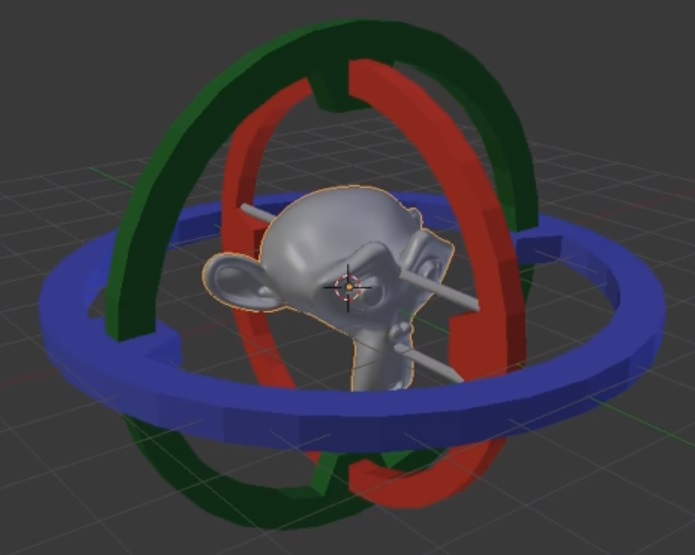
\includegraphics[width=.9\linewidth]{Figures/euler-1.jpg}
  \caption{Posizione neutra.}
  \label{fig:eulerA}
\end{subfigure}%
\begin{subfigure}{.5\textwidth}
  \centering
  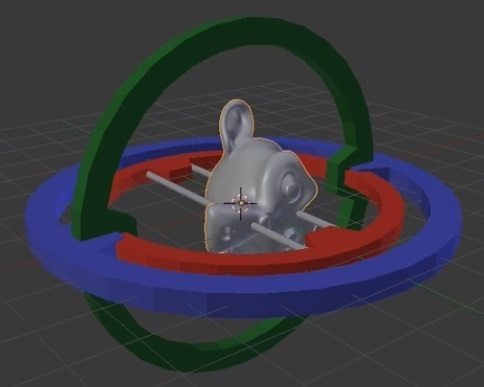
\includegraphics[width=.9\linewidth]{Figures/euler-2.jpg}
  \caption{Gimbal lock, l'asse X e Z sono allineati.}
  \label{fig:eulerB}
\end{subfigure}
\decoRule
\caption[Rotazione Euleriana]{Rappresentazione di rotazione Euleriana attraverso un giroscopio a tre assi.}
  \begin{minipage}{.8\textwidth}
  \footnotesize
  \emph{(Immagini di Nathan Vegdahl)}
  \end{minipage}
\label{fig:euler}
\end{figure}

Concettualmente è la più intuitiva di tutte: utilizza 3 assi di rotazione (X, Y, Z) ed il funzionamento è analogo a quello di un giroscopio. ogni asse offre un DOF, quindi sono possibili rotazioni con 3 DOF. Tuttavia sono necessarie due accortezze: 
\begin{enumerate}
    \item ordine degli assi;
    \item gimbal lock problem.
\end{enumerate}
L'ordine degli assi è decisivo, in quanto quello più interno dipende dalla rotazione di quelli esterni. Di conseguenza ruotando gli assi in un ordine diverso da quello specificato porta a risultati diversi da quello atteso. In più, interpolazioni tra diversi orientamenti, possono a loro volta risultare sgradevoli, poiché la rotazione viene spezzata in 3 movimenti.

Il problema del gimbal lock \parencite{anticz16}, in italiano blocco cardanico, sorge dall'allineamento di due assi: quello più interno e quello più esterno. Ne deriva che ruotano uno di questi 2 assi si ottiene la stessa rotazione, perdendo quindi un DOF.
È quindi importante scegliere l'ordine degli assi in maniera tale che il primo e il terzo non risultino mai allineati.

Per ovviare a questo problema può essere conveniente bloccare uno degli assi in una posizione fissa. Per questo motivo, la forma Euleriana è meglio utilizzata nelle giunture con 1 o 2 DOF.

\newpage
\subsection{Quaternione}
\begin{figure}[ht]
\centering
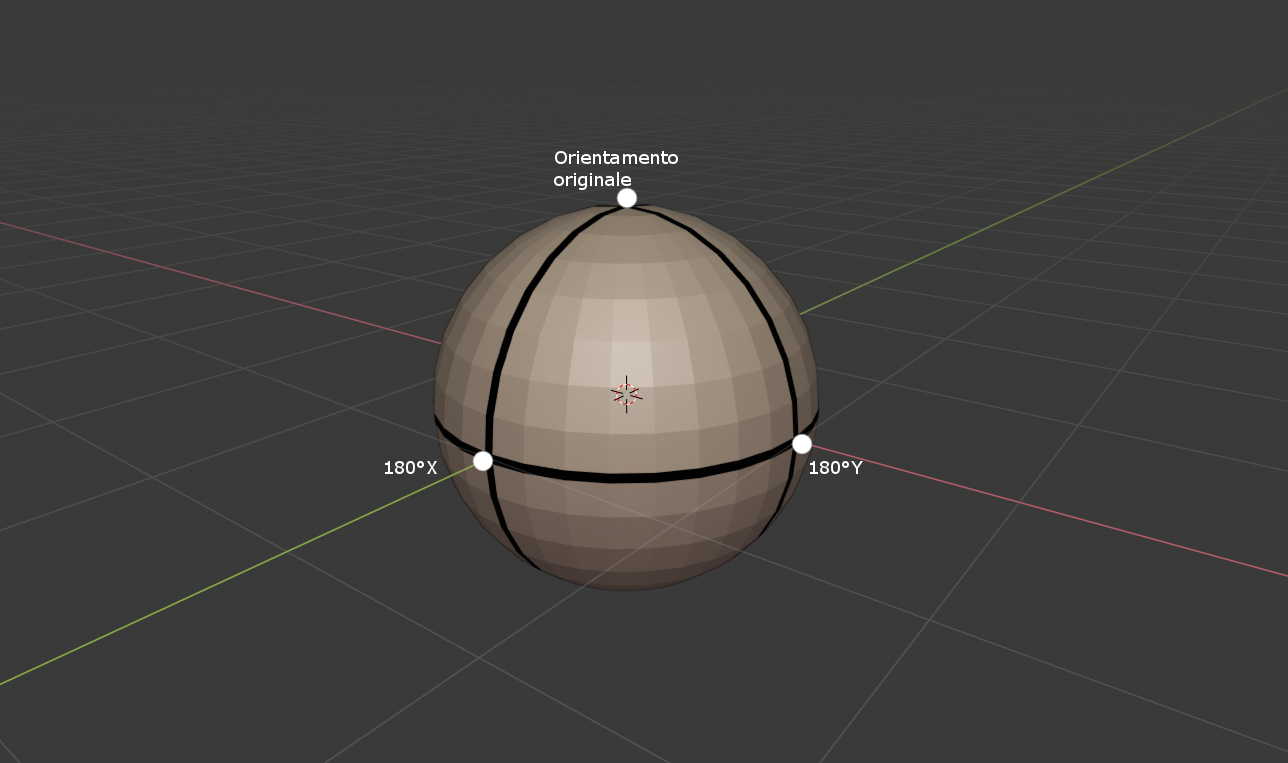
\includegraphics[width=.8\textwidth]{Figures/3d-sphere}
\decoRule
\caption[Quaternione 2D]{Rappresentazione di un quaternione 2D su una sfera 3D.}
\label{fig:quater}
\end{figure}
In contrasto a quanto appena visto, la forma di quaternione è concettualmente complessa, ma in pratica diventa molto utile e senza molti dei difetti della controparte Euleriana.

I principali benefici della rappresentazione a quaternione includono l'eliminazione del gimbal lock. Infatti è presente una componente in più, ma ciascuna componente non rappresenta un asse quanto piuttosto l'orientamento dell'oggetto ruotato intorno a quell'asse. La quarta componente serve quindi a definire la posizione neutra.

L'interpolazione risulta diretta e dolce, infatti il movimento non è spezzato sui diversi assi e l'ordine di questi non è importante. Infine rende comodo calcolare una rotazione opposta semplicememte invertendo il segno della componente W.

Per rendere tutto ciò possibile servono 4 componenti (X, Y, Z, W), come già detto in precedenza, uno per la posizione originale più una per la rotazione su ogni asse. Se si prende il caso di rotazioni su due assi si può immaginare che queste 3 componenti siano 3 punti su una sfera, come mostrato in Figura \ref{fig:quater}. Ogni altra rotazione è data dall'interpolazione di questi tre punti.

La ragione per cui i due punti sulla sfera rappresentano una rotazione di 180\textdegree\ anziché 90\textdegree\ e resa necessaria siccome altrimenti questi due punti coinciderebbero nel punto più basso della sfera. Come effetto aggiuntivo è possibile rappresentare rotazioni fino a 720\textdegree\ ed ogni orientamento equivale a due possibili rotazioni dando all'animatora l'abilità di decidere in che verso ruotare l'oggetto durante un'animazione. 

\subsection{Matriciale}
Quest'ultima è probabilmente la rappresentazione più ottimale in termini di flessibilità, in quanto permette di rappresentare anche traslazioni, scalature e altre trasformazioni come \emph{shear}. È, infatti, la rappresentazione che blender utilizza internamente \cite{blendApi} \cite{nat2012rig} proprio perché offre la maggior flessibilità.

Siccome permette di rappresentare qualsiasi tipo di trasformazione, questa struttura viene solitamente chiamata \emph{Matrice di Trasformazione}. Nel caso di uno spazio a 3 dimensioni, essa ha dimensione $4\times4$.

Questa sua caratteristica la rende indispensabile per rappresentare articolazioni formate da più ossa (i.e Kinematics Linkages) che verranno illustrati qui di seguito (sezioni \ref{sectionFK} e \ref{sectionIK}), poiché rende possibile convertire le coordinate locali di un osso (rappresentato in Figura \ref{fig:FK}, evidenziato in azzurro) figlio a quelle locali del suo padre, fino ad arrivare alle coordinate globali.

L'unico difetto è che, come la rappresentazione sotto forma di quaternione, non mantiene l'informazione sul percorso della rotazione. Infatti è ancora più simile a una delta-rotazione (i.e. differenza di orientamento), rispetto ad un quaternione poiché copre una rotazione di soli 360\textdegree, rispetto ai 720\textdegree\ del quaternione. 

\newpage
\section{Cinematica Diretta} \label{sectionFK}

\begin{figure}
\centering
\begin{subfigure}{.33\textwidth}
  \centering
  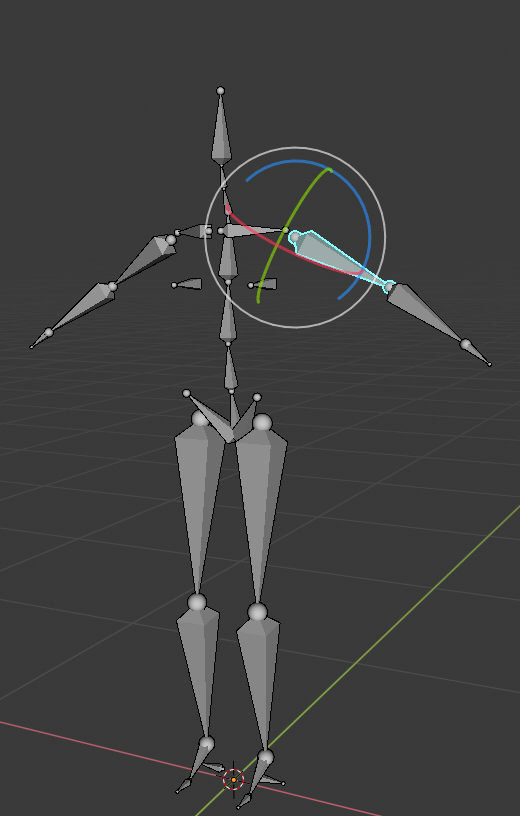
\includegraphics[width=\linewidth]{Figures/armature1}
  \label{fig:FK1}
\end{subfigure}%
\begin{subfigure}{.33\textwidth}
  \centering
  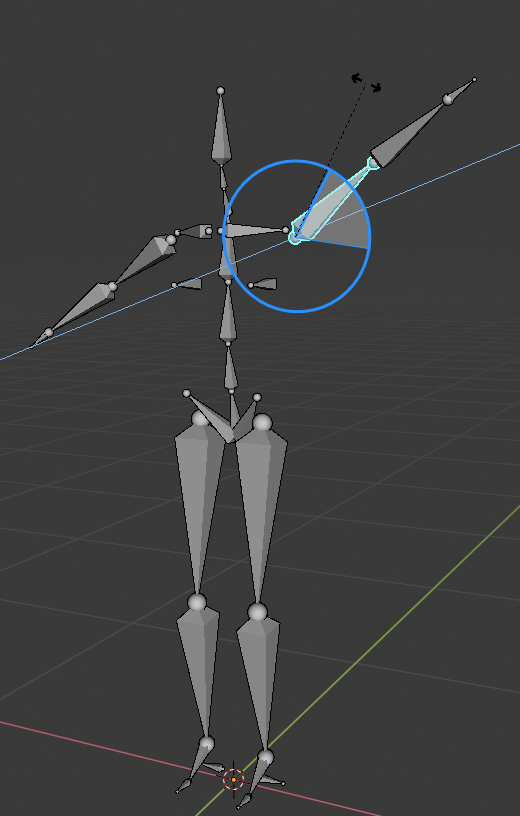
\includegraphics[width=\linewidth]{Figures/armature2}
  \label{fig:FK2}
\end{subfigure}%
\begin{subfigure}{.33\textwidth}
  \centering
  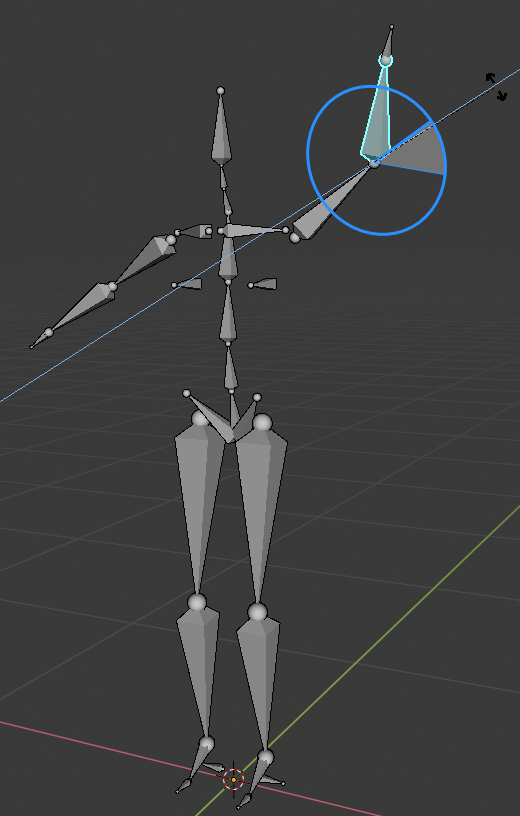
\includegraphics[width=\linewidth]{Figures/armature3}
  \label{fig:FK3}
\end{subfigure}
\decoRule
\caption[Cinematica Diretta]{Esempio di posizionamento tramite Forward Kinematic. La figura rappresenta la stessa armatura, formata da diverse ossa, in tre posizioni differenti.}
\label{fig:FK}
\end{figure}

Per figure complesse, come quella umana (da qui in avanti tutti gli esempi saranno riferiti alla figura umana, siccome, nella realizzazione del corto, è stata il centro della maggior parte delle animazioni), è utile avere un sistema che permetta di posizionare le sue componenti in maniera relativa ad altre. Per esempio, una volta posizionato il busto, posizionare il braccio, poi la mano ed in fine le dita, tutto in maniera relativa a quanto posizionato in precedenza.

Questa tecnica permette infatti di specificare, attraverso una rotazione, la posizione di un osso relativa al suo osso padre. Per questo motivo serve che le ossa di un'armatura (vedi Figura \ref{fig:FK}) siano organizzate in maniera gerarchica (i.e. ad albero). In questo modo, quando l'armatura viene posizionata basterà moltiplicare tutte le matrici di trasformazione dalla radice ai nodi foglia in maniera \emph{deep-first}. 
Per definire una posa è quindi necessario specificare la rotazione di ogni osso. Questo permette un controllo preciso su ogni DOF dell'armatura, il che è ottimo, perché permette all'animatore di realizzare pose perfette, senza lasciare che nulla venga calcolato automaticamente. 

Lo svantaggio è che questa metodologia rende difficile animare azioni comuni in cui gli arti si muovono in uno spazio non relativo al resto del corpo, ma rispetto allo spazio circostante. Ad esempio, per aprire una porta tenendo la mano sulla maniglia, il corpo si può spostare di lato, ma la mano deve rimanere aggrappata alla maniglia. Con una metodologia FK, l'animatore dovrebbe infatti spostare il corpo e, ogni volta, riposizionare la mano sulla maniglia, introducendo un sacco di \emph{counter-animation}, ovvero l'animazione inversa per riposizionare la mano nella posizione in cui era prima del movimento del resto del corpo.

\section{Cinematica Inversa} \label{sectionIK}

\begin{figure}
\centering
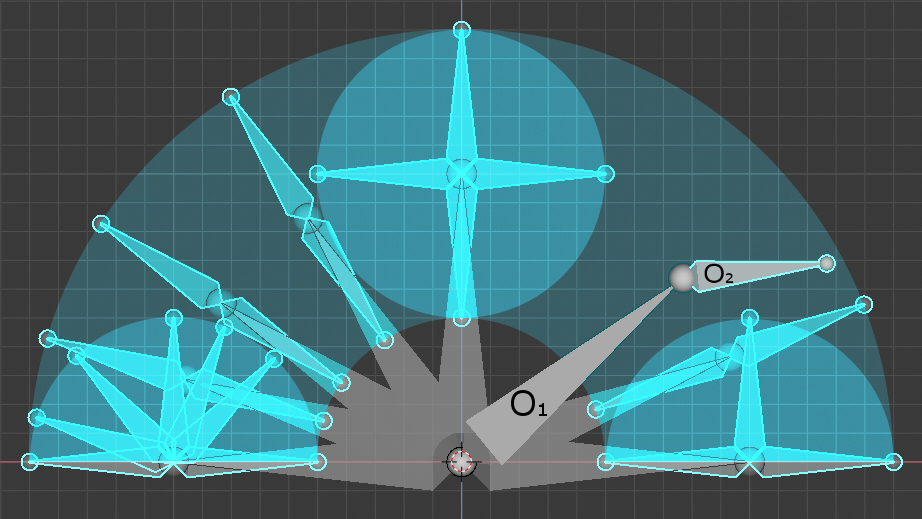
\includegraphics[width=.8\textwidth]{Figures/2Dlinkage}
\decoRule
\caption[Inverse Kinematic 2D]{Esempio di segmento di scheletro formato da due ossa in uno spazio 2D. Quello evidenziato in azzurro è lo spazio raggiungibile dall'\emph{end-effector}}
\label{fig:IK}
\end{figure}

Il concetto di Inverse Kinematic è, fondamentalmente l'inverso di Forward Kinematic. In quest'ultimo ogni osso influenza la rotazione di quelli che lo seguono (i.e. figli).
Al contrario, in IK, muovere un osso alla fine di una sequenza (i.e. \emph{end-effector}), influenza la posizione di quelli che lo precedono.
Ciò è molto utile nel caso in cui si vogliano posizionare gli arti di una figura umana, in quanto rende il tutto più intuitivo.
IK serve anche a fare in modo che una serie di ossa mantenga un estremo (i.e. \emph{end-effector}) connesso a qualcosa.
Definite la posizione della mano e della radice (spalla) la posizione delle ossa intermedie viene calcolata automaticamente.
Esistono diverse tecniche per il calcolo degli angoli delle articolazioni intermedie.

Nel caso di articolazioni relativamente semplici è possibile calcolare l'intero spazio delle soluzioni analiticamente, ed individuare tra esse quelle che soddisfano l'obiettivo.
Ad esempio, nel caso di un sistema di due ossa ($O_1$ e $O_2$) e due articolazioni in uno spazio 2D come in Figura \ref{fig:IK} lo spazio raggiungibile dall'\emph{end-effector} può essere descritto come 
\begin{equation*}
    \{x: |O_1-O_2| \leq x \leq O_1+O_2\}
\end{equation*}
\newpage
Data la posizione $(X,Y)$ obiettivo dell'\emph{end-effector}, se questa cade all'interno dello spazio raggiungibile, è possibile attraverso le formule trigonometriche, ricavare gli angoli delle 2 articolazioni:
\begin{align}
    \arccos{ (\theta _T) } &=  \frac{X}{\sqrt{X^2+Y^2}}\\
    \theta_T &= \arccos{\left(  \frac{X}{\sqrt{X^2+Y^2}} \right)}\\
    \cos{( \theta_1-\theta_T )} &=  \frac{O_1^2+X^2+Y^2-O_2^2}{2O_1\sqrt{X^2+Y^2}}\\
    \theta_1 &= \arccos{\left(  \frac{O_1^2+X^2+Y^2-O_2^2}{2O_1\sqrt{X^2+Y^2}}\right)}+\theta_T\\
    \cos{(180-\theta_2)} = -\cos{(\theta_2)} &= \frac{O_1^2+O_2^2-(X^2+Y^2)}{2O_1O_2}\\
    \theta_2 &= \arccos{\left(\frac{O_1^2+O_2^2-X^2+Y^2}{2O_1O_2}\right)}
\end{align}

Nell'equazioni sopra riportate $\theta_1$ e $\theta_2$ si riferiscono agli angoli rispetto alla posizione naturale dei rispettivi ossi. $\theta_T$ è l'angolo formato dall'ipotenusa immaginaria che si forma tracciando un segmento dalla radice alla posizione obiettivo dell'end-effector, rispetto alla posizione naturale di $O_1$.

Per casi più complessi, come spesso capita nelle animazioni digitali, viene usato un metodo iterativo  analogo alla risoluzione di un problema di ottimizzazione in programmazione lineare \cite{lp2017}.
Ciò consiste nel ricalcolare gli angoli di tutte le articolazioni ad ogni passo dell'iterazione, fino ad arrivare alla posizione obiettivo.
Per fare ciò viene usata una matrice di derivate parziali chiamata matrice Jacobiana \cite{Parent:2012:CAA:2385444} che ha la seguente struttura.

\[J=
\begin{bmatrix}
    \dfrac{\partial p_x}{\partial \theta_1} & \dfrac{\partial p_x}{\partial \theta_2} & \dots & \dfrac{\partial p_x}{\partial \theta_n} \\[2ex]
    \dfrac{\partial p_y}{\partial \theta_1} & \dfrac{\partial p_y}{\partial \theta_2} & \dots & \dfrac{\partial p_y}{\partial \theta_n} \\[2ex]
    \dfrac{\partial p_z}{\partial \theta_1} & \dfrac{\partial p_z}{\partial \theta_2} & \dots & \dfrac{\partial p_z}{\partial \theta_n} \\[2ex]
    \dfrac{\partial \alpha_x}{\partial \theta_1} & \dfrac{\partial \alpha_x}{\partial \theta_2} & \dots & \dfrac{\partial \alpha_x}{\partial \theta_n} \\[2ex]
    \dfrac{\partial \alpha_y}{\partial \theta_1} & \dfrac{\partial \alpha_y}{\partial \theta_2} & \dots & \dfrac{\partial \alpha_y}{\partial \theta_n} \\[2ex]
    \dfrac{\partial \alpha_z}{\partial \theta_1} & \dfrac{\partial \alpha_z}{\partial \theta_2} & \dots & \dfrac{\partial \alpha_z}{\partial \theta_n} 
\end{bmatrix}
\]

Questa matrice è formata da tante colonne quante sono le articolazioni. Ciascun vettore colonna è poi costituito da 6 componenti, 3 ($x$, $y$ e $z$) per la posizione ($p$) e altre 3 per l'orientamento ($\alpha$).
La funzione obiettivo è data da...

Blender propone anche un metodo alternativo per risolvere la cinematica inversa che tiene conto anche di altri vincoli definiti dall'utente \cite{blendDoc}. Questo metodo si chiama iTaSC e, come il metodo standard, utilizza una matrice Jacobiana, ma il modo in cui la calcola è diverso \cite{blendWiki}.

Un motivo per cui il metodo iterativo è migliore di quello analitico, oltre ad essere l'unico metodo per risolvere articolazioni complesse, è che, nel caso in cui la posizione obiettivo si trovi al di fuori dello spazio raggiungibile, (e.g. la mano deve raggiungere un punto troppo distante dalla spalla) non esiste nessuna soluzione e in questo caso il risultato può e dev'essere approssimato.

Siccome quello della cinematica inversa è un problema sotto-vincolato, è molto probabile che esista più di una soluzione. Nel caso visto in Figura \ref{fig:IK} ad esempio esistono 2 soluzioni, per un qualsiasi punto $(X,Y)$ interno allo spazio raggiungibile, simmetriche rispetto alla linea immaginaria che collega la radice di $O_1$ alla punta di $O_2$.
In tal caso il risultato è scelto dall'algoritmo tra una delle possibili soluzioni. Non sempre però, sono tutte realistiche o visivamente gradevoli.
Per questo motivo è possibile aggiungere dei vincoli per limitare il numero di soluzioni possibili, molto utili sono quelli per l'imitare il movimento di un arto, per renderlo più realistico.


